%%%%%%%%%%%%%%%%%%%%%%%%%%%%%%%%%%%%%%%%%
% University/School Laboratory Report
% LaTeX Template
% Version 3.1 (25/3/14)
%
% This template has been downloaded from:
% http://www.LaTeXTemplates.com
%
% Original author:
% Linux and Unix Users Group at Virginia Tech Wiki 
% (https://vtluug.org/wiki/Example_LaTeX_chem_lab_report)
%
% License:
% CC BY-NC-SA 3.0 (http://creativecommons.org/licenses/by-nc-sa/3.0/)
%
%%%%%%%%%%%%%%%%%%%%%%%%%%%%%%%%%%%%%%%%%

%----------------------------------------------------------------------------------------
%	PACKAGES AND DOCUMENT CONFIGURATIONS
%----------------------------------------------------------------------------------------

\documentclass{article}

\usepackage{array}
\usepackage{tabularx}
\usepackage{geometry}
\usepackage{graphicx} % Required for the inclusion of images
\usepackage[utf8]{inputenc}
\usepackage[english]{babel}
\usepackage{minted}
\usemintedstyle{borland}
\usepackage{xcolor}
\setlength\parindent{1.2pt} % Removes all indentation from paragraphs

\renewcommand{\labelenumi}{\alph{enumi}.} % Make numbering in the enumerate environment by letter rather than number (e.g. subsection 6)
\geometry{
 a4paper,
 total={170mm,257mm},
 left=20mm,
 top=20mm,
 }
%\usepackage{times} % Uncomment to use the Times New Roman font

%----------------------------------------------------------------------------------------
%	DOCUMENT INFORMATION
%----------------------------------------------------------------------------------------

\title{
	Microcontroller Lab Report \\
\large 8086 programming Part 2a
} % Title

\author{
	Aaditya Prakash Kattekola \\
	{\small Roll: 194201} \\
	{\small ECE Section B} \\
} % Author name

\date{August 28, 2021} % Date for the report

\begin{document}

\maketitle % Insert the title, author and date

% If you wish to include an abstract, uncomment the lines below
% \begin{abstract}
% Abstract text
% \end{abstract}

%----------------------------------------------------------------------------------------
%	Question 1
%----------------------------------------------------------------------------------------

\break
\section{Question 1}
%----------------------------------------------------------------------------------------
%	subsection 1
%----------------------------------------------------------------------------------------

\subsection{Aim}
Write an efficient assembly language program (minimum code length) for 8086 MP for a system has four inputs and four outputs. The four output bits represents the gray code equivalent of input binary number.
%----------------------------------------------------------------------------------------
%	subsection 2
%----------------------------------------------------------------------------------------

\subsection{Program}
\subsubsection{Code}
\inputminted{nasm}{"C:/Users/aadit/Documents/BTech/5th Semester/MC Lab/8086 Pgrm 2/2A/GRAY_CODE.asm"}

\subsubsection{Emulator}

\begin{center}
\begin{tabularx}{1.0\textwidth} { 
  | >{\centering\arraybackslash}X 
  | >{\centering\arraybackslash}X 
  | >{\centering\arraybackslash}X | }
 \hline
\textbf{Address  (CS:0100, IP:0000)} &\textbf{Machine code}&\textbf{Instruction} \\
  \hline
 01000 & B8,0B,00 & MOV AX, 0000BH \\ 
  \hline
   01003 & 8B, D8 & MOV BX, AX \\ 
  \hline
   01005 & D1, E8 & SHR AX, 1 \\  
  \hline
  01007 & 33, C3 & XOR AX, BX \\  
  \hline
 01009 & F4 & HLT \\  
  \hline
\end{tabularx}
\end{center}

%----------------------------------------------------------------------------------------
%	subsection 3
%----------------------------------------------------------------------------------------
\break
\subsection{Result}
\subsubsection{Input}
AX: 1011B  (B in HEX) \\

\subsubsection{Expectation}
$AX \leftarrow 
AX \oplus BX; \\  
1011B+0101B \rightarrow 1110B \ or \ 000EH \ in \ AX$ \\

%----------------------------------------------------------------------------------------
%	subsection 4
%----------------------------------------------------------------------------------------

\subsubsection{Emulator}

\begin{figure}[h]
\begin{center}
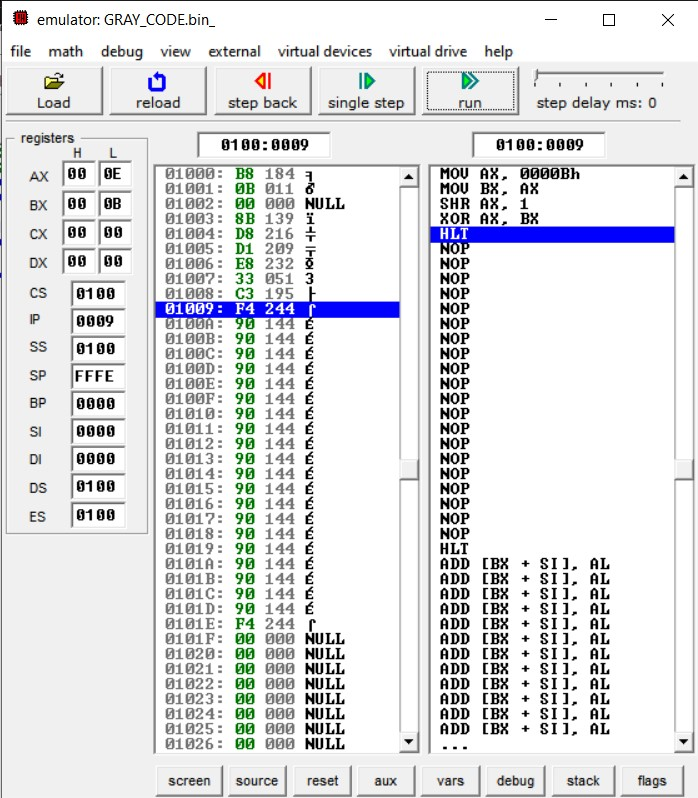
\includegraphics[width=0.8\textwidth]{GRAY_OUT} 
\caption{STACK Output for Q1}
\end{center}
\end{figure}


%----------------------------------------------------------------------------------------
%	Question 2
%----------------------------------------------------------------------------------------

\break
\section{Question 2}
%----------------------------------------------------------------------------------------
%	subsection 1
%----------------------------------------------------------------------------------------

\subsection{Aim}
Write a program for 8086 processor to generate the Fibonacci series (Each number in the Fibonacci series is the sum of the previous two numbers.)
%----------------------------------------------------------------------------------------
%	subsection 2
%----------------------------------------------------------------------------------------

\subsection{Program}
\subsubsection{Code}
\inputminted{nasm}{"C:/Users/aadit/Documents/BTech/5th Semester/MC Lab/8086 Pgrm 2/2A/FIBONACCI.asm"}

\subsubsection{Emulator}

\begin{center}
\begin{tabularx}{1.0\textwidth} { 
  | >{\centering\arraybackslash}X 
  | >{\centering\arraybackslash}X 
  | >{\centering\arraybackslash}X | }
 \hline
\textbf{Address  (CS:0100, IP:0000)} &\textbf{Machine code}&\textbf{Instruction} \\
  \hline
 01000 & B0, 00 & MOV AL, 00H \\ 
  \hline
   01002 & BE, 00, C9 & MOV SI, 0C900H \\ 
  \hline
  01005 & 88, 04 & MOV [SI], AL \\ 
  \hline
01007 & 46 & INC SI \\ 
  \hline
  01008 & FE, C0 & INC AL \\
  \hline
  0100A & 88, 04 & MOV [SI], AL \\	  
  \hline
  0100C & B1, 05 & MOV CL, 05H \\
  \hline
  0100E & 80, E9, 02 & SUB CL, 02H \\
  \hline
  01011 & 8A, 44, FF & MOV AL, [SI] - 01H \\
  \hline
  01014 & 02, 04 & ADD AL, [SI] \\
  \hline
  01016 & 46 & INC SI \\
  \hline
  01017 & 88, 04 & MOV [SI], AL \\
  \hline
  01019 & FE, C9 & DEC CL \\
  \hline
  0101B & FE, C9 & JNE 011H \\
  \hline
 0101D & F4 & HLT \\  
  \hline
\end{tabularx}
\end{center}

%----------------------------------------------------------------------------------------
%	subsection 3
%----------------------------------------------------------------------------------------
\break
\subsection{Result}
\subsubsection{Input}
CL: 05H ;LENGTH OF FIBONACCI SERIES

\subsubsection{Expectation}

$ SI \leftarrow C900H \\
\lbrack C900 \rbrack :  00 \, \  
\lbrack C901\rbrack: 01 \\
\lbrack SI + 1 \rbrack \leftarrow 
\lbrack SI  \rbrack + \lbrack SI - 1 \rbrack \\  
0100:C900\ \ \  00\ 01\ 01\ 02\ 03
$ 

%----------------------------------------------------------------------------------------
%	subsection 4
%----------------------------------------------------------------------------------------

\subsubsection{Emulator}
\begin{figure}[h]
\begin{center}
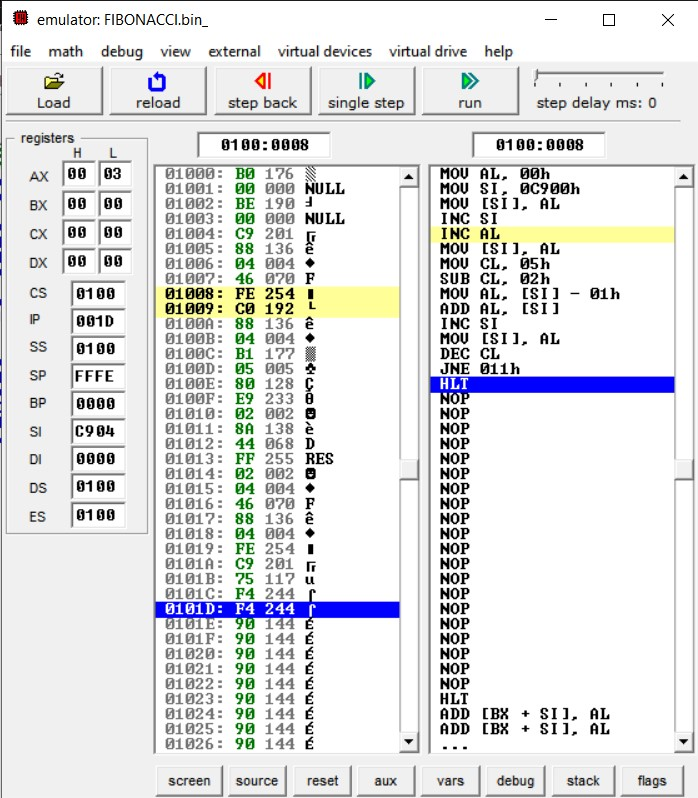
\includegraphics[width=0.65\textwidth]{FIB_OUT1} 
\caption{STACK Output for Q2}
\end{center}
\begin{center}
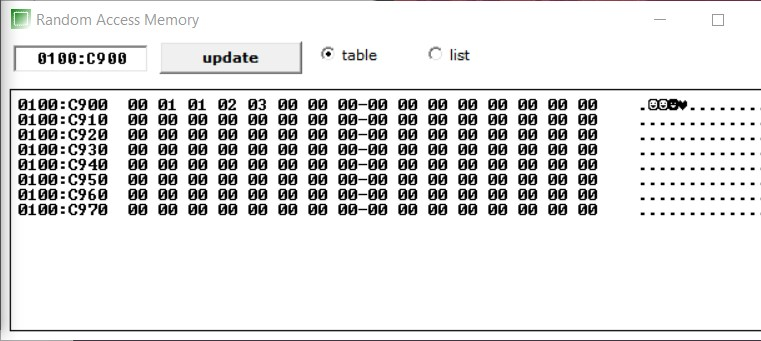
\includegraphics[width=0.55\textwidth]{FIB_OUT2} 
\caption{RAM Output for Q2}
\end{center}
\end{figure}

\end{document}